\documentclass{article}
\usepackage[english]{babel}
\usepackage[a4,top=2cm,bottom=2cm,left=3cm,right=3cm,marginparwidth=1.75cm]{geometry}
\usepackage{amsmath}
\usepackage{graphicx}
\usepackage[colorlinks=true, allcolors=blue]{hyperref}

\title{Project 1: Inference of BK initial condition}
\author{Carlisle Aurabelle Casuga}

\begin{document}
\maketitle

\section{MV}

For the initial run on the MV model with 50 design points, sampled using plain latin hypercube sampling within a wide parameter  space with bounds: $Q_{s0}²$ = [0.001, 2.0] 1/GeV²; $C²$ = [0.1, 100.0], and $\sigma_{0}/2$ = [1.0, 40.0] mb, the following results were obtained: 

\begin{figure}[h]
\centering
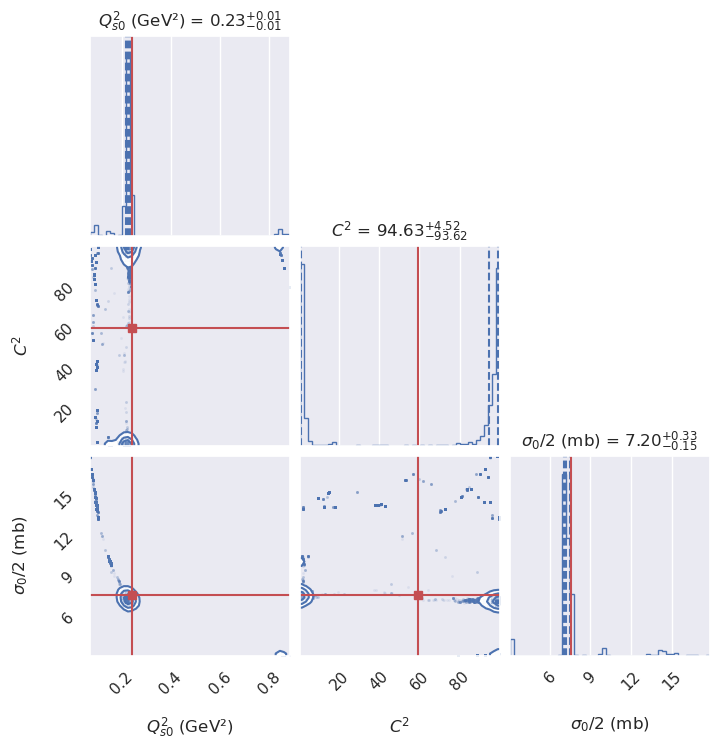
\includegraphics[width=0.5\textwidth]{figs\mv_50d_initial_50w.png}
\caption{Initial run on the MV model with 50 design points}
\label{fig:mv_50d_50w}
\end{figure}

Figure \ref{fig:mv_50_1} is sampled with 50 walkers, total 1500 steps, 500 of which are burn steps. This will provide us with a rough estimate of the posterior distribution of the parameters. Actual values of the parameters at the 16\%, 50\%, and 84\% percentiles are:

$Q_{s0}²$: [(0.16, 0.21728015544863194), (0.5, 0.2275510190337838), (0.84, 0.23450182482460977)]
$C²$: [(0.16, 1.0035763833397198), (0.5, 94.62810202727259), (0.84, 99.14833702805878)]
$\sigma_{0}/2$: [(0.16, 7.052807276014379), (0.5, 7.200058879152208), (0.84, 7.5276927226268135)]

From the 2013 paper, the values of the parameters are: $Q_{s0}²$ = 0.104 GeV²; $C²$ = 14.5, and $\sigma_{0}/2$ = 18.2 mb. We have a large disparity between these values and the values we obtained from the initial run. Next run we can tighten the bounds of $Q_{s0}²$ = [0.001, 0.5] but widen the C² parameters to [0.05, 150.0] to accomodate the peak at large values of C².

We show here the chain of walkers in this run where some of the walkers are stuck in areas of low likelihood. To resolve this, we  double the number of walkers to 100 and run the sampler for 1000 burn steps. Then we (emcee) sample within a tighter space surrounding the posterior distribution peaks. 

\begin{figure}[h]
\centering
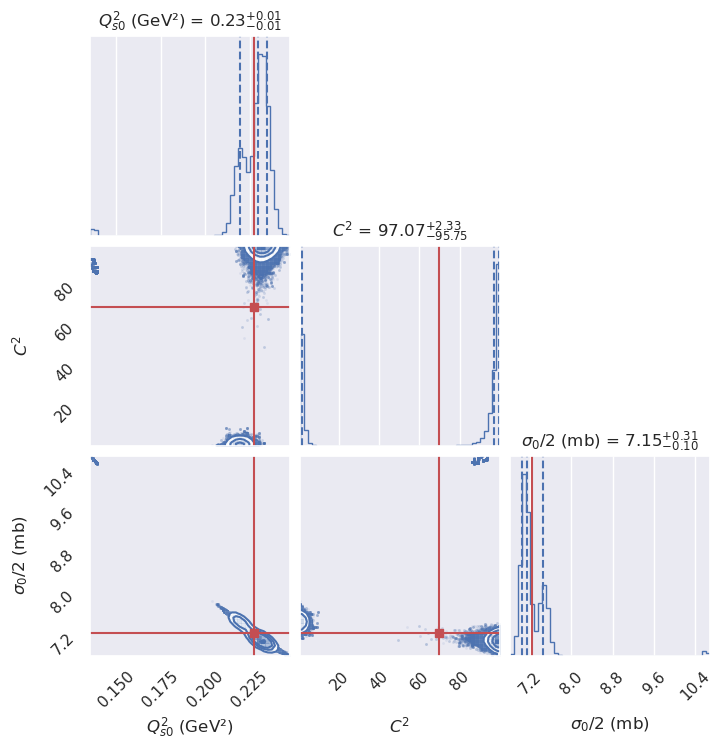
\includegraphics[width=0.5\textwidth]{figs\mv_50d_initial_100w.png}
\caption{Same MV run but with 100 walkers}
\label{fig:mv_50d_100w}
\end{figure}

\section{MVe}

With the MVe model, there are 4 free model parameters to be fitted against: $$Q_{s0}²$$ $$C²$$ $$\sigma_{0}/2$$ with the addition of $$e_c$$. The bounds of the LHS sampling of the parameters are: $Q_{s0}²$ = [0.001, 2.0] 1/GeV²; $C²$ = [0.1, 100.0], and $\sigma_{0}/2$ = [1.0, 40.0] mb. The bounds of $e_c$ are [0.5, 100.0]. In this run we aimed to sample 49 design points through both plain LHS and orthogonal LHS. In both cases the GPE performed very poorly with very large errors and off predictions. The next run is to try with more design points, specifically 121 design points.

The GPE is ran with an RBF + WhiteKernel kernels and whose initial hyperparameters were set at "length_scale = 1 * np.ones(theta.shape[1]), length_scale_bounds = (1e-10, 1e10)" but with the Whitekernel with default parameters. We also set n_restart_optimizer = 2 so that a better fit is made. With these settings there is no error warning regarding the determination of the optimal hyperparameter of the kernels. With 10\% of the training data as validation data and n=5 principal components, the GPE produces the following predictions for a single kinematical point. We also show  the zscore for a single kinematical point.

\begin{figure}[h]
\centering
\includegraphics[width=0.5\textwidth]{figs\mve_121d_gpe.png}
\caption{GPE predictions for a single kinematical point}
\label{fig:mve_121d_gpe}
\end{figure}

\begin{figure}[h]
\centering
\includegraphics[width=0.5\textwidth]{figs\mve_121d_zscore.png}
\caption{Zscore for a single kinematical point}
\label{fig:mve_121d_zscore}
\end{figure}

The emcee sampling for 100 walkers (30 minutes run time) is performed and from the chain, the walkers were not properly converged as we can see from the chain plot. We run the sampler again for more walkers (500) and less $Q_s0²$ space, in the hopes of finding a better convergence. Unfortunately, we show here that it does converge the walkers but nonetheless a poor sampling distribution is obtained. 

\begin{figure}[h]
\centering
\includegraphics[width=0.5\textwidth]{figs\mve_121d_500w.png}
\caption{MVe run with 500 walkers}
\label{fig:mve_121d_500w}
\end{figure}

with quantile values
Quantiles: [(0.16, 0.10444113262841531), (0.5, 0.1100391634489063), (0.84, 0.16343216074397923)]
Quantiles: [(0.16, 12.423226137980059), (0.5, 65.03766366566634), (0.84, 66.67212300526586)]
Quantiles: [(0.16, 15.868392244095453), (0.5, 48.19438130661283), (0.84, 81.1793240923539)]
Quantiles: [(0.16, 5.978122615546301), (0.5, 6.203794380396528), (0.84, 6.79909337149499)]

To further prove that this is not a good sampling run, the mean acceptance is 0.197. The optimal acceptance ratio is .2 to .5.

I had a suspicion on whether there was something wrong with generating the training set. However, when I tried using the same code to generate the training set for past runs, there was no problems. Let's compare the bayesian sampling in both cases. The first one is the old training set while the second one the new one. There is no difference in the sampling distribution besides the old one just had more samples. So there was no weird change to the training set code.

\begin{figure}[h]
\centering
\includegraphics[width=0.5\textwidth]{figs\4p_new.png}
\caption{tight MVe run with old training set}
\label{fig:4p_new}
\end{figure}

\begin{figure}[h]
\centering
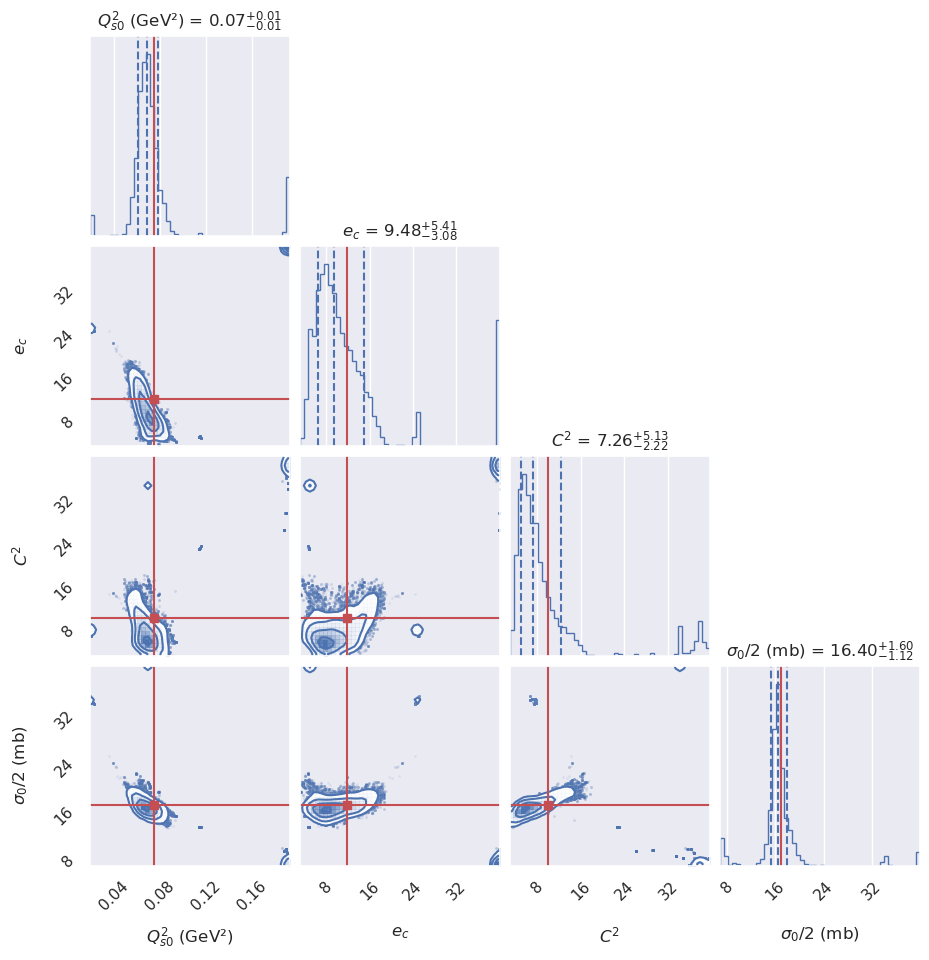
\includegraphics[width=0.5\textwidth]{figs\4p_new_vs.png}
\caption{tight MVe run with new training set}
\label{fig:4p_new_vs}
\end{figure}

I had the idea of combining a past MVe run with this current one. This old run has LH samples within a tighter parameter space where $Q_{s0}²$ = [0.001, 0.2] 1/GeV²; $e_c$ = [0.5, 40.0] ; $C²$ = [0.1, 40.0], and $\sigma_{0}/2$ = [1.0, 40.0] mb. This involved generating a training set from Q² = 2.0 GeV² to 10 GeV² to cover what was lacking in the old run and then combining the two training sets and parameter vector sets. So that a wider array of training data and parameter values (denser in the tighter region) can give us the areas where the likelihood is maximized. (Theta file and training file was appended).

The sampling distribution is shown below. 

Quantiles: [(0.16, 0.06739340877316732), (0.5, 0.11670826980103077), (0.84, 0.21280114410076745)]
Quantiles: [(0.16, 11.079119769318801), (0.5, 60.1650779980113), (0.84, 99.0661828030286)]
Quantiles: [(0.16, 9.1138629738339), (0.5, 14.641110632950689), (0.84, 65.43275805593659)]
Quantiles: [(0.16, 4.765888420339204), (0.5, 6.945807097304044), (0.84, 17.08536031618019)]

\begin{figure}
\centering
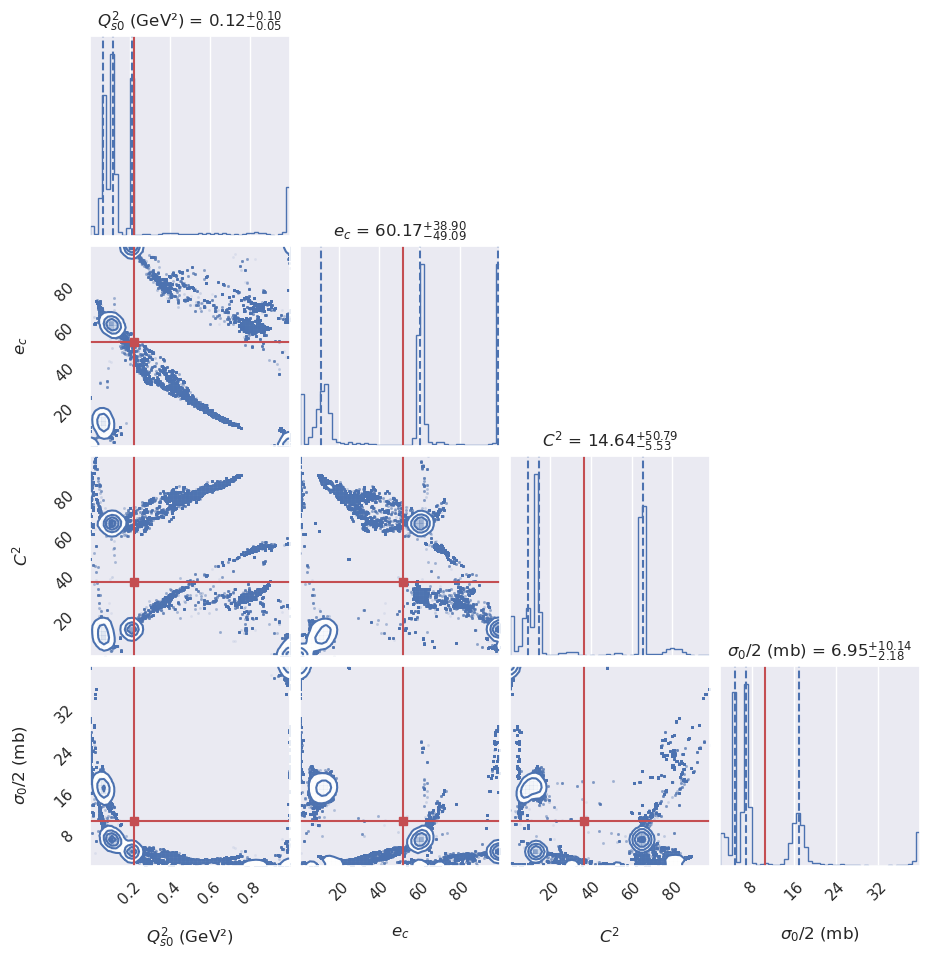
\includegraphics[width=0.5\textwidth]{figs\mve_121+100d_500w.png}
\caption{MVe run with 500 walkers with hybrid training set}
\label{fig:mve_121+100d_500w}
\end{figure}

\begin{figure}
\centering
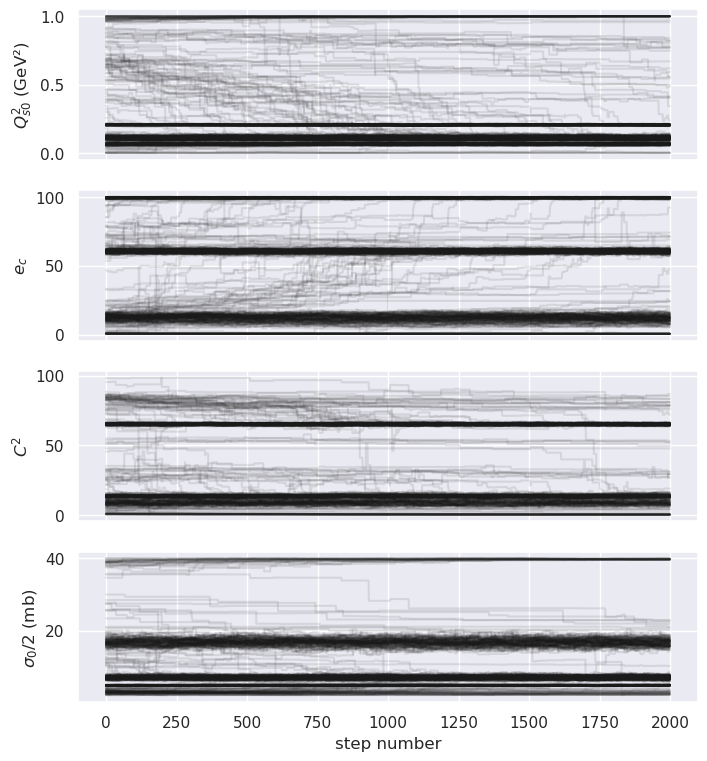
\includegraphics[width=0.5\textwidth]{figs\mve_121+100d_500w_chain.png}
\caption{MVe run with 500 walkers with hybrid training set: chain}
\label{fig:mve_121+100d_500w_chain}
\end{figure}

\begin{figure}
\centering
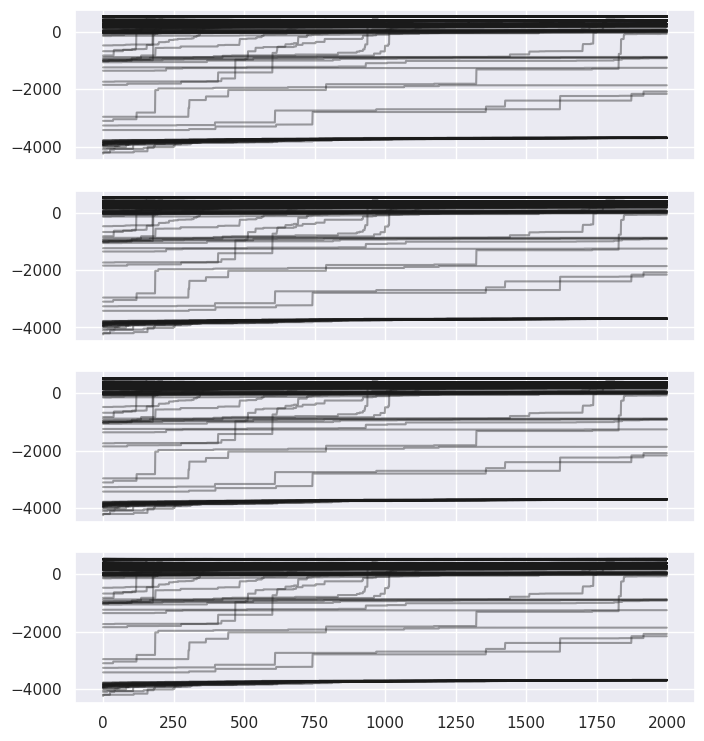
\includegraphics[width=0.5\textwidth]{figs\mve_121+100d_500w_logprob.png}
\caption{MVe run with 500 walkers with hybrid training set: log prob}
\label{fig:mve_121+100d_500w_logprob}
\end{figure}

\begin{figure}
\centering
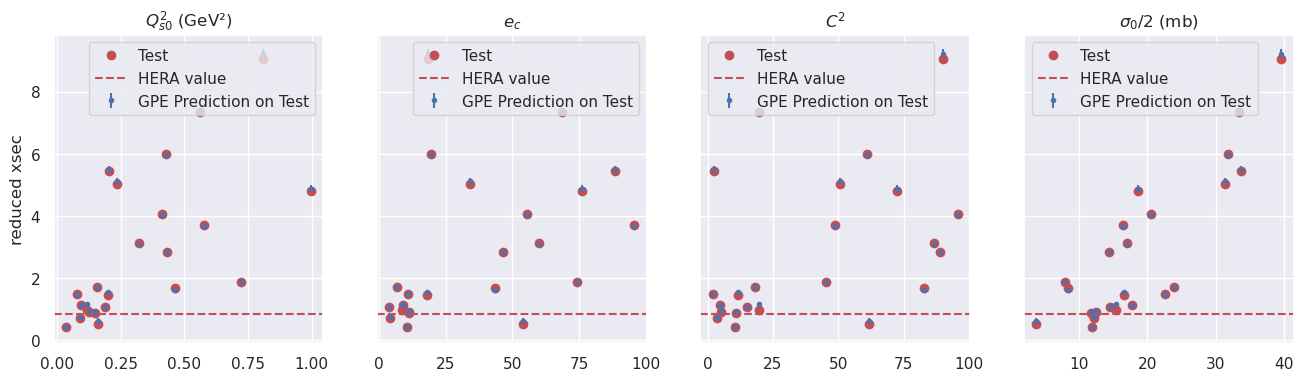
\includegraphics[width=0.5\textwidth]{figs\mve_121+100d_gpe.png}
\caption{GPE prediction at a single kinematical point}
\label{fig:mve_121+100d_gpe}
\end{figure}

Even if the GPE is performing well, because the walkers were initialized in a very large space, they struggle to find the optimal likelihood spots. Despite converegences at localized spots, the log prob chain shows that they settle at different values of posterior probabilities. The 1d and 2d histograms shown are therefore not very reliable. 

Let's try it again with a smaller initialization space and less walkers.

\begin{figure}
\centering
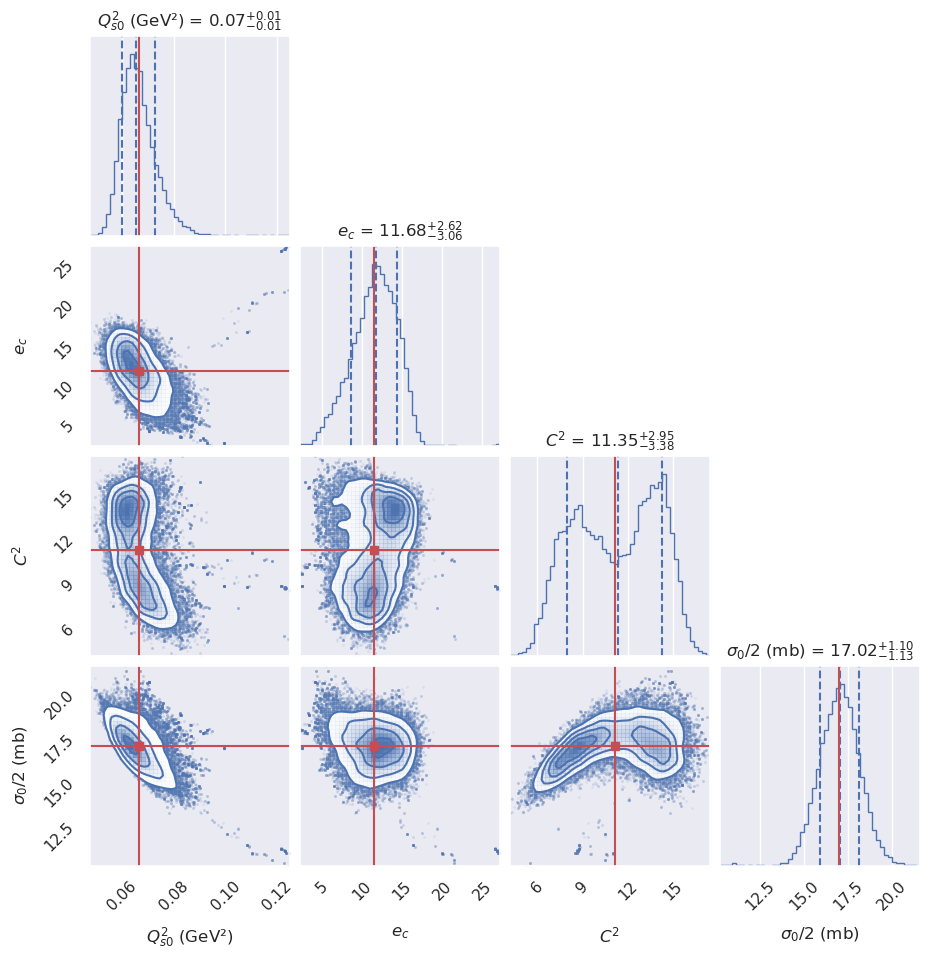
\includegraphics[width=0.5\textwidth]{figs\mve_121+100d_100w_narrow.png}
\caption{MVe run with 100 walkers with hybrid training set}
\label{fig:mve_121+100d_100w_narrow}
\end{figure}

This shows proper convergence in both posterior distributions and sample chain. However, there is no proper peak for the C² posterior distribution. I tried setting a narrower initialization for the other parameters and set C² to be initialized at a wider bound [0.1, 100.0] but that did not help as can be seen below.

\begin{figure}
\centering
\includegraphics[width=0.5\textwidth]{figs\mve_121+100d_100w_narrowinit_wideC2.png}
\caption{MVe run with 100 walkers with hybrid training set: C² initialized at [0.1, 100.0]}
\label{fig:mve_121+100d_100w_narrowinit_wideC2}
\end{figure}

So far we have not been able to constrain C². Next, I have a suspicion that training the gpe for such a wide parameter space messes up the correlations between the values of the reduced cross section. So we switch back to the complete training set but with training set generated with design points sampled in a narrower bound where $Q_{s0}²$ = [0.001, 0.2] 1/GeV²; $e_c$ = [0.5, 40.0] ; $C²$ = [0.1, 40.0], and $\sigma_{0}/2$ = [10.0, 30.0] mb, a more reasonable space centered around the values found in the rcbk paper. 

The GPE was trained for 403 kinematical points where the Q^2 range is from 2.0 to 50.0 GeV^2 where the BK limit is valid. The GPE prediction did very well with 10 percent test data and 6 principal components chosen via qualitative scan of the z-score for different number of components shown below:

\begin{figure}
\centering
\includegraphics[width=0.5\textwidth]{figs\mve_100d_zscore.png}
\caption{Z-score for different number of principal components}
\label{fig:mve_100d_zscore}
\end{figure}

And this is how the GPE performs for a single kinematical point. 

\begin{figure}
\centering
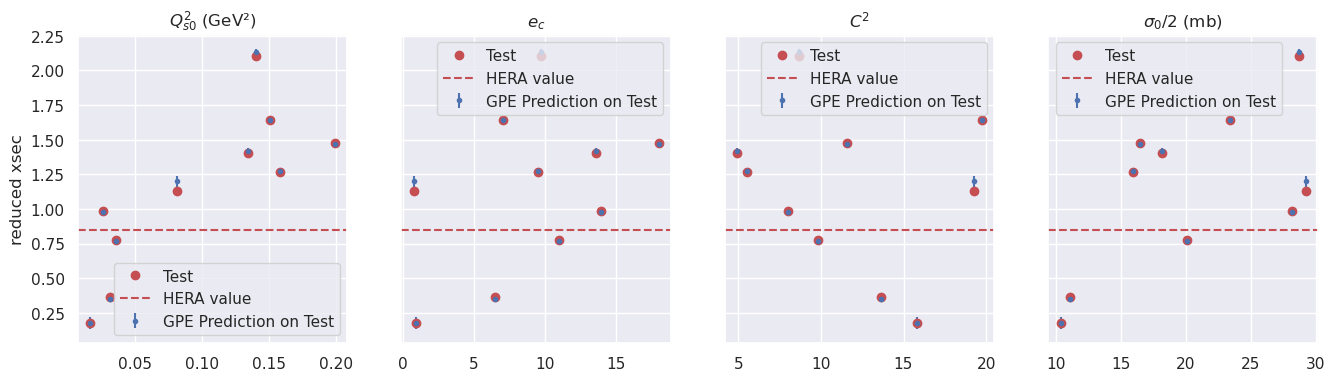
\includegraphics[width=0.5\textwidth]{figs\mve_100d_gpe.png}
\caption{GPE prediction at a single kinematical point}
\label{fig:mve_100d_gpe}
\end{figure}

And this is how the emcee sampling went (using 100 walkers, 2000 burn steps and 1000 production steps):

\begin{figure}
\centering
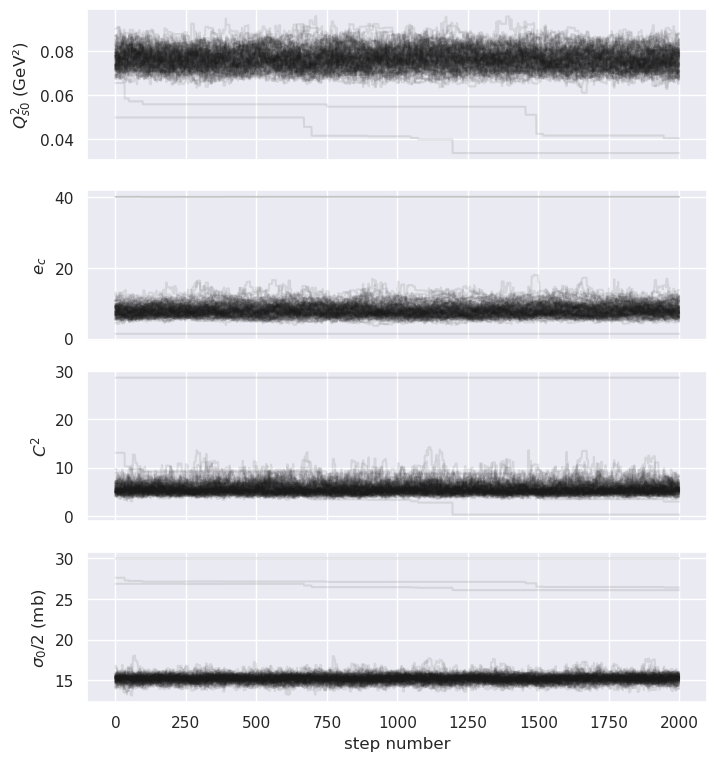
\includegraphics[width=0.5\textwidth]{figs\mve_100d_100w_chain.png}
\caption{MVe run with 100 walkers with design points that have smaller parameter space: chain}
\label{fig:mve_100d_100w_chain}
\end{figure}

\begin{figure}
\centering
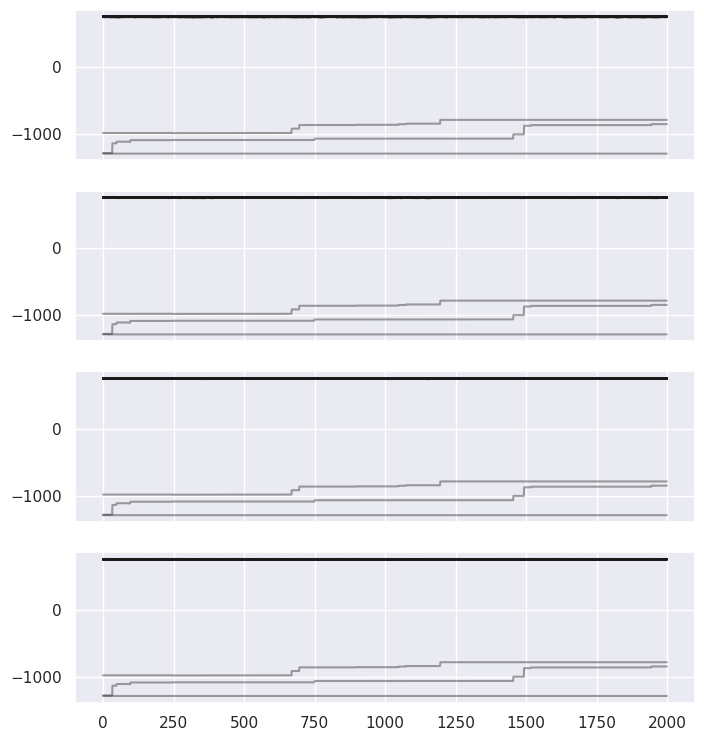
\includegraphics[width=0.5\textwidth]{figs\mve_100d_100w_logprob.png}
\caption{MVe run with 100 walkers with design points that have smaller parameter space: log prob}
\label{fig:mve_100d_100w_logprob}
\end{figure}

\begin{figure}
\centering
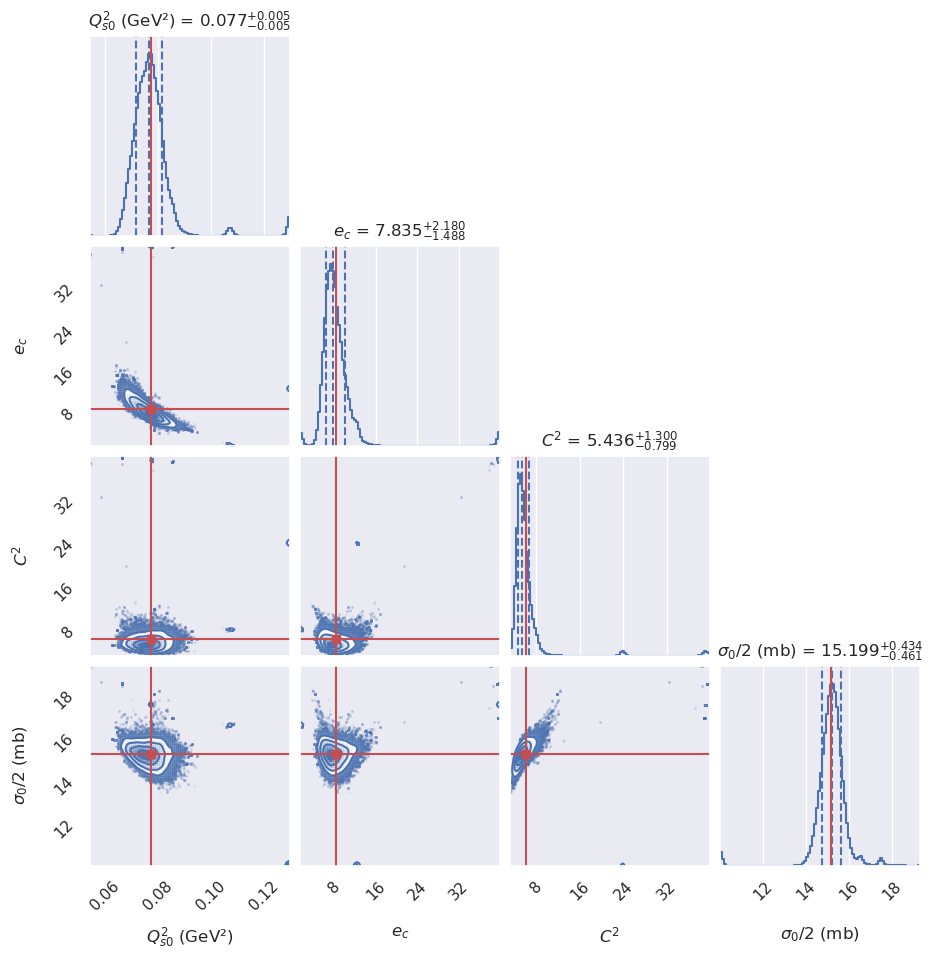
\includegraphics[width=0.5\textwidth]{figs\mve_100d_100w.png}
\caption{MVe run with 100 walkers with design points that have smaller parameter space}
\label{fig:mve_100d_100w}
\end{figure}

As can be seen, this is reliable because the values have converged pretty nicely. These plots have quantile values at:

Quantiles: [(0.16, 0.07167898754863827), (0.5, 0.07659888520137269), (0.84, 0.08143020768290565)]
Quantiles: [(0.16, 6.3469525054075735), (0.5, 7.834631953247264), (0.84, 10.01465421992532)]
Quantiles: [(0.16, 4.636596860991138), (0.5, 5.436055036040134), (0.84, 6.73622171023949)]
Quantiles: [(0.16, 14.737995258738518), (0.5, 15.199272555845912), (0.84, 15.633713579507749)]

Mean and acceptance fraction:
$Q_{s0}^{2}$ (GeV²)= 0.077
$e_c$= 8.417
$C^{2}$= 6.192
$\sigma_0/2$ (mb)= 15.173
Mean acceptance fraction: 0.400

Sampling over an even narrower parameter space to remove the outlier walkers give us the following:

\begin{figure}
\centering
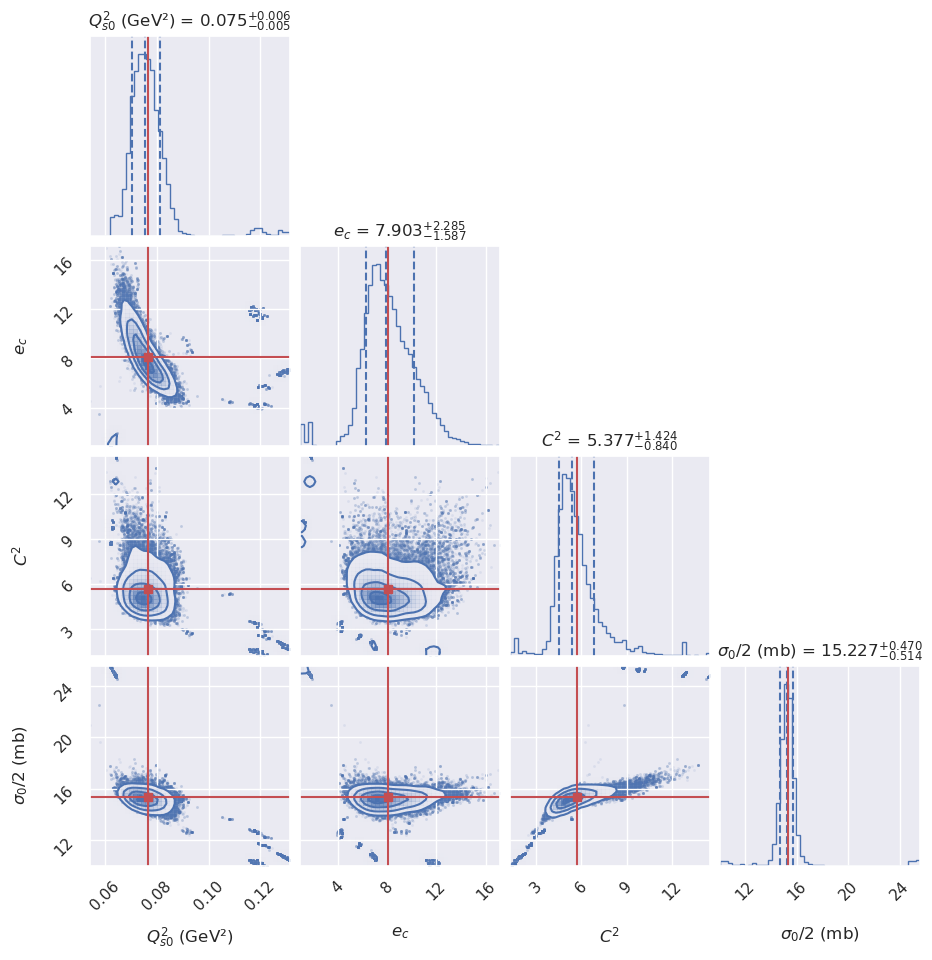
\includegraphics[width=0.5\textwidth]{figs\mve_100d_100w_narrow.png}
\caption{MVe run with 100 walkers with design points that have even smaller parameter space}
\label{fig:mve_100d_100w_narrow}
\end{figure}

Quantiles: [(0.16, 0.07042138348378785), (0.5, 0.0754394360116123), (0.84, 0.0812312219535772)]
Quantiles: [(0.16, 6.315976026500409), (0.5, 7.902611886718099), (0.84, 10.187421279951657)]
Quantiles: [(0.16, 4.5375863981247), (0.5, 5.377111454170131), (0.84, 6.800972081221537)]
Quantiles: [(0.16, 14.713371518080658), (0.5, 15.227200628204383), (0.84, 15.696835034938939)]

$Q_{s0}^{2}$ (GeV²)= 0.077
$e_c$= 8.107
$C^{2}$= 5.674
$\sigma_0/2$ (mb)= 15.318
Mean acceptance fraction: 0.371

I would prefer the first one because it has a higher acceptance fraction and better convergence.

One hundred parameter vectors are now obtained from these posterior distributions (saved in "mve_100d_100w_sampled_from_posterior.txt" file) and obtained model cross sections from these samples. These values are ploted against experimental data. Say, for example, at Q2 = 45.0 GeV and sqrt(s) = 318.0 GeV, we compare the training set vs 100 design points sampled in the posterior.

\begin{figure}
\centering
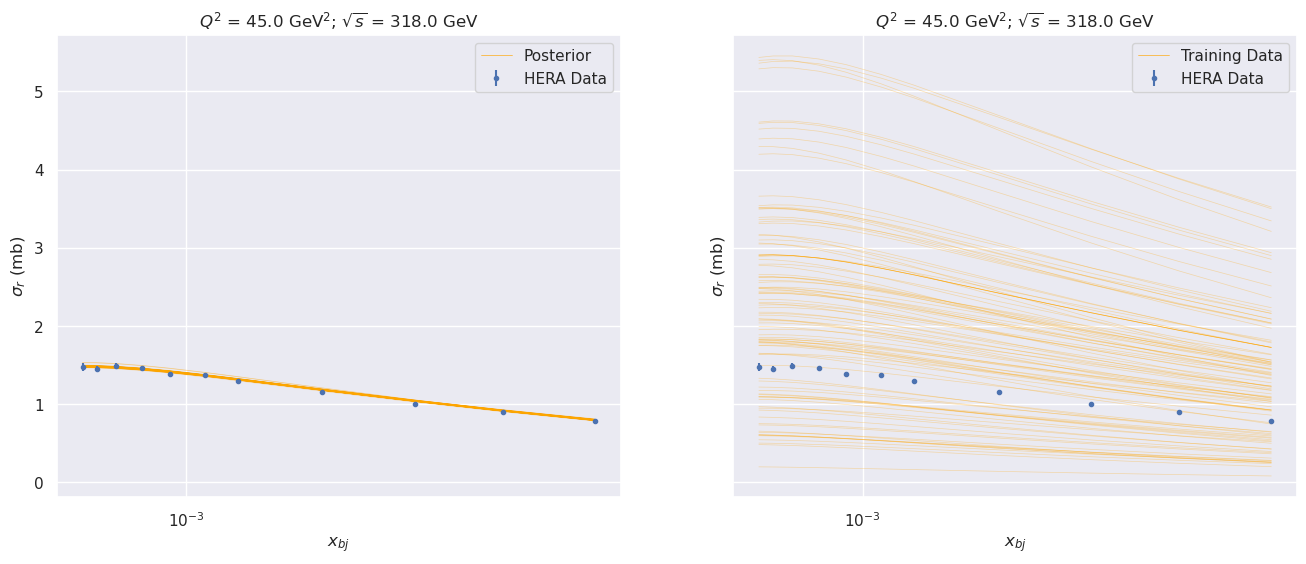
\includegraphics[width=0.5\textwidth]{figs\mve_train_vs_post_45_318.png}
\caption{Training set vs posterior samples at Q2 = 45.0 GeV and sqrt(s) = 318.0 GeV}
\label{fig:mve_train_vs_post_45_318}
\end{figure}

\end{document}